
\begin{comment}
Because multithreaded programs frequently use updates to shared memory to communicate, \dthreads{} must implement a mechanism to expose one thread's updates to all other threads.  At the beginning of a transaction, all shared pages are protected, and can only be read by threads.  When a thread attempts to modify a shared page a local working copy is created, leaving the shared page unmodified.  At commit time, a ``twin'' copy of all modified pages is created.  Every page is compared to its twin (using a byte-wise diff) and modified bytes are copied back to the shared state.  Unlike transactional memory, conflicting changes do not result in rollbacks with \dthreads{}.  Further details are described in Section~\ref{sec:sharedmemory}.
\end{comment}


\label{sec:dthreads-architecture}
This section describes \dthreads{}’ key algorithms---isolated execution, deterministic (diff-based) memory commit, deterministic synchronization, and deterministic memory allocation---as well as other implementation details.

\begin{figure}
{\centering 
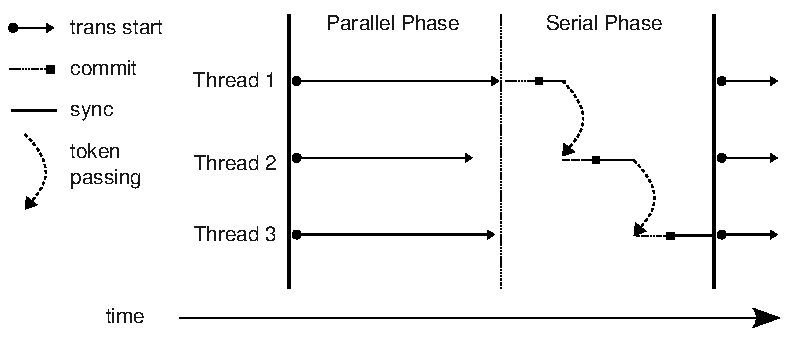
\includegraphics[width=6in]{dthreads/figure/phase}
\caption{An overview of \dthreads{} phase. Program execution with \dthreads{} alternates between parallel and serial phases.\label{fig:phase}}
}
\end{figure}

Figure~\ref{fig:phase} illustrates the execution of programs under \dthreads{}. \dthreads{} divides the execution of each thread into alternating parallel phases and serial phases. 
Based on the \sheriff{} framework, \dthreads{} isolates memory accesses in parallel phases. These accesses work on private copies of memory; that is, updates are not shared between threads during the parallel phases. When a synchronization point is reached, updates are applied (or made visible) in a deterministic order, as well as synchronizations. 
  
\subsection{Isolated Execution}
\label{sec:threadsasprocs}

Relying on the \sheriff{} framework (Section~\ref{sec:sheriffframework}), \dthreads{} turns threads into processes, with separate address spaces but the shared file table (Section~\ref{sec:threadcreat}). Thus, \dthreads{} isolates memory accesses among different threads between synchronization points: different threads can only see their own local changes. Those changes are merged together at synchronization points in order to achieve the shared memory semantics. Those details to achieve this target are discussed in Section~\ref{sec:sharedmemory}.  

\subsection{Deterministic Memory Commit}
\label{sec:sharedmem}

This section describes the mechanisms used to guarantee deterministic commit order, and the details of commits to the shared memory. These mechanisms are not provided by the \sheriff{} framework.   

\subsubsection{Fence and Token}
\label{sec:schedule}

\dthreads{} places internal fences between parallel and serial phases. \dthreads{} re-implements the fence because the standard \pthreads{}'s barrier mechanism does not support dynamic changes of threads number. 

\begin{figure}
\begin{lstlisting} [style=tt]
void waitFence(void) {
  lock();
	
  while(!isArrivalPhase()) { 
    CondWait();
  }

  waiting_threads++;
  if(waiting_threads < alive_threads) {
    while(!isDeparturePhase()) {
      CondWait();
    }
  } 
  else {
    setDeparturePhase();
    CondBroadcast();
  }

  waiting_threads--;
  if (waiting_threads == 0) {
    setArrivalPhase();
    CondBroadcast();
  }

  unlock();
}

\end{lstlisting}
\caption{Pseudocode for the internal fence.\label{fig:internalFence}}
\end{figure}

Figure~\ref{fig:internalFence} shows the pseudocode code for the internal fence. Threads must wait at an internal conditional variable until all threads departed from the last departure phase (lines 4-5). Then those threads are waiting at the fence until all alive threads have arrived at the same fence (lines 8-11). The last thread initiates the departure phase and wakes up all threads on the conditional variable (lines 14-15). As threads leave the fence, they decrement the number of waiting threads.  The last thread to leave sets the fence to the arrival phase and wakes any waiting threads (lines 19-21).

To reduce overhead, whenever the number of running threads is less than or equal to the number of cores, waiting threads use spin locks, instead of expensive cross-process \pthreads{} mutexes. When the number of threads exceeds the number of cores, \dthreads{} falls back to using \pthreads{} mutexes.

\begin{figure}
\begin{lstlisting} [style=tt]
void waitToken() {
  waitFence();
  while(isNotMyToken()) { yield(); }
}
void putToken() {
  passTokenToNextOfTokenQueue();
}
\end{lstlisting}
\caption{Pseudocode for waitToken and putToken. 
\label{fig:token}}
\end{figure}

Another key mechanism of \dthreads{} is the global token, which \dthreads{} uses to order memory commits and synchronizations. The token implementation is listed in Figure~\ref{fig:token}. The token is a shared pointer that points to the next runnable thread entry, which guarantees the global order for all operations in serial phases.  

\dthreads{} introduces two subroutines to manage tokens.  The \texttt{waitToken()} function first waits at the internal fence and then waits to acquire the global token in order to enter or leave the serial phases. The \texttt{putToken()} function passes the token to the next waiting thread. 

As shown in Figure~\ref{fig:phase}, it is very important for a thread to wait at the internal fence before a thread enters  or leaves serial phases, even for a thread that is guaranteed to have the token next. Otherwise, memory commits of a thread can affect other threads' behavior, bringing non-determnism. 

\subsubsection{Commit Protocol}

Figure~\ref{fig:architecture} shows the steps to track modifications to the shared state and expose them in a deterministic order.  

At the beginning of parallel phases, different threads have a read-only mapping for all shared pages. If a thread writes to a shared page during a parallel phase, this write is trapped in order to create a private copy and a twin page for this shared page. After that, reads and writes on this page happen on the private copy only. For those non-trapped pages, reads go directly to the shared state.  

In serial phases, threads first commit their local changes that happen in last parallel phase, guided by the global token.  The first thread to commit to a page can directly copy its private working copy to the shared state (page-based commits), but subsequent commits can only commit the modified bytes (byte-based commits) using the diffing mechanism discussed in Section~\ref{sec:twinning-and-diffing}. The byte-based commits are much slower than the page-based commits, but  they won't overwritten changes committed by previous threads.  After a thread commits its local changes, it issues synchronizations before it passes the token to its next thread. 

In the end of serial phases, every thread has to recover the read-only mapping and wait at the internal fence before enterring into the next parallel phase. 

\subsection{Deterministic Synchronization}
\label{sec:synchronization}

\dthreads{} supports the full range of synchronizations of \pthreads{} APIs, including locks, conditional variables, barriers and different types of thread exits. Since the \sheriff{} framework can not provide any deterministic guarantee, \dthreads{} implements different types of synchronizations in a deterministic way, discussed in the following sections. 

\subsubsection{Locks}
Before a thread acquires a lock, it has to wait for the global token, by calling \texttt{waitToken}. 

\dthreads{} treats multiple locks as the same one. It only ends the current serial phase for a thread when all locks held by this thread are unlocked. Thus, it is possible for a program with deadlock problems that those deadlocks do not occur to \dthreads{} at all. 

At acquisitions of locks, \dthreads{} checks at first whether the current thread is already holding any locks. If not, the thread first waits for the token, commits those changes happened in the last parallel phase to the shared state, and begins a new atomic section. Finally, the thread increments the number of locks that it is currently holding. The lock count ensures that a thread does not pass the token to the next one until it has released all of the locks.

During releases of locks, \dthreads{} decrements the lock count at first. A thread does nothing if there are still some locks holding by the current thread, with the lock count not equal to 0. If all locks have been released, \dthreads{} commits the memory changes happened in this serial phase to the shared state. Then it passes the global token to the next thread of the token queue and waits on the internal fence before entering into the next round's parallel phase.

\subsubsection{Condition Variables}
\label{sec:condwait}

Guaranteeing determinism for condition variables is much more complex than for other synchronization primitives. The underlying operating system can not guarantee that threads are going to be waken-up in the same order as their waits. Thus, a naive implementation easily leads to a no-progress problem if the first waken-up thread can not get the global token to proceed first.

When a thread calls \texttt{pthread\_cond\_wait}, it first acquires the global token and commits local modifications that happen during this serial phase since \texttt{pthread\_cond\_wait} is generally issued inside a critical section. It then removes itself from the token queue since threads waiting on condition variables do not participate in the token pass until they are awakened. Then, \dthreads{} adds itself to the conditional variable's waiting queue, decreases the number of alive threads (used in the internal fence mechanism), and passes the token to the next thread on the token queue before actually waiting on a process-shared conditional variable. 

When a thread is awaken, it should check at first whether the current thread is ready to run or not. For the deterministic reason, \texttt{pthread\_cond\_signal} should only wake up the first thread waiting on a conditional variable but the operating system, like Linux, can not guarantee this. Thus, we specifically wake up all threads, but only the first thread is given the permission to run. If a thread is not able to run, it waits on this conditional variable again; if a thread is the candidate thread to be waken up, it waits for the global token to enter into the next serial phase, which this thread should get immediately in order to avoid a no-progress problem. 

For \texttt{pthread\_cond\_signal} and \texttt{pthread\_cond\_broadcast}, the calling thread first waits for the global token, and then commits any local modifications before issuing an actual wake-up signal. If no threads are waiting on a condition variable, \dthreads{} passes the token to the next thread immediately. Otherwise, \dthreads{} migrates corresponding threads, one for \texttt{pthread\_cond\_signal} and all for \texttt{pthread\_cond\_broadcast}, in the condition variable queue to the head of the token queue, marks them as ready, and increments the number of alive threads correspondingly. 


\subsubsection{Barriers}

\label{sec:barrierwait}

Threads waiting on a barrier should not disrupt the token passing of running threads: \dthreads{} removes threads entering into the barrier from the run queue and places them on the corresponding barrier queue.

In order to ensure determinism, the calling thread first waits for the global token to commit any local modifications. If the current thread is the last one to enter the barrier, \dthreads{} moves all threads on the barrier queue to the token queue, increases the number of alive threads, and passes the token to the first thread in the barrier queue. Otherwise, \dthreads{} removes the current thread from the token queue, places it on the barrier queue, releases the token, and waits on the actual barrier.


\subsubsection{Thread Creation and Exit}

\label{sec:threadcreation}

\begin{figure}
\begin{lstlisting} [style=tt]
void thread_create () {
  waitToken();
  clone(CLONE_FS| CLONE_FILES | CLONE_CHILD);
  if(isChild) {
    allocGlobalThreadIndex();
    insertToTokenQueue();
    notifyChildRegistered();
	// Wait for the parent to reach next sync point
    waitParentBroadcast();	
  }
  else if (isParent) {
    waitChildRegistered();
  }
}
\end{lstlisting}
\begin{lstlisting} [style=tt]
void thread_exit() {
  waitToken();
  atomicEnd(false);
  removeFromTokenQueue();
  decreaseInternalFence();
  putToken();
  exitThread(); 
}
\end{lstlisting}
\caption{Pseudocode for thread creation and exit($\S$~\ref{sec:threadcreation}).
\label{fig:threadcreation}
}
\end{figure}

To guarantee determinism, thread creations and exits must be performed in serial phases. 

For performance reason, a thread is allowed to create multiple threads without waiting for a new serial phase, thus improving the parallelism. Figure~\ref{fig:threadcreation} shows the pseudocode for thread creation and thread exit. The calling thread firstly waits for the token before proceeding (line 2). It then creates a new process with shared file descriptors but a distinct address space using the \texttt{clone} system call (line 3).  Then the parent thread is waiting until its child thread has registered itself. 

The newly created child obtains the global thread index (line 5), places itself in the token queue (line 6), and notifies the parent that child has registered itself in the token queue(line 7). To proceed, the child thread then waits for the parent to reach the next synchronization point.  Thus, we can allow a parent thread to create multiple children threads in the same serial phase. 

When \texttt{thread\_exit()} is called, the caller first waits for the token and then commits any local modifications (line 3). It then removes itself from the token queue (line 4) and decreases the number of alive threads (line 5). Finally, the thread passes its token to the next thread in the token queue (line 6) and exits (line 7).

\subsubsection{Thread Cancellation}

\dthreads{} performs thread cancellations in serial phases in order to guarantee determinism. A thread can only invoke \texttt{pthread\_cancel} while holding the global token. If the thread being cancelled is waiting on a condition variable or a barrier, it is removed from the queue deterministically. Finally, to cancel a thread, \dthreads{} kills the target process using kill(tid, SIGKILL) and decrements the number of alive threads after the cancellation.

\subsection{Deterministic Memory Allocation}
Programs sometimes rely on the addresses of objects returned by the memory allocator intentionally (for example, by hashing objects based on their addresses), or accidentally. A program with a memory error, like a buffer overflow, will yield different results for different memory layouts.

The reliance on memory addresses can undermine other efforts to provide determinism. For example, CoreDet is unable to fully enforce determinism because it relies on the Hoard scalable memory allocator~\cite{Bergan:2010:CCR:1736020.1736029}. Hoard was not designed to provide determinism and several of its mechanisms, thread id based hashing and non-deterministic assignment of memory to threads, lead to nondeterministic execution in CoreDet for the Canneal benchmark. To resolve this problem, \dthreads{} employs both deterministic thread index and custom memory allocation mechanism. 

\subsubsection{Deterministic Thread Index}
\label{sec:threadindex}

POSIX does not guarantee deterministic process or thread identifiers. To avoid exposing this nondeterminism to threads that run as processes, \dthreads{} shims the \texttt{pthread\_self()} function in order to return an deterministic thread index.  This thread index is managed using a single global variable that is incremented on every thread creation.  This unique thread index is also used to manage per-thread heaps and as an offset into an array of thread entries.

\subsubsection{Custom Memory Allocation}

To preserve determinism in the face of intentional or inadvertent reliance on memory addresses, we designed the \dthreads{} memory allocator to be fully deterministic. 

\dthreads{} assigns subheaps to each thread based on its deterministically assigned thread index. In addition to guarantee the same mapping of threads to subheaps on different executions, \dthreads{} allocates superblocks (large chunks of memory) deterministically by acquiring a lock (and the global token) on each superblock allocation. Thus, threads always use the same subheaps, and these subheaps always acquires the same superblocks on each execution. The superblocks themselves are allocated via mmap: while \dthreads{} could use a fixed address mapping for the heap, we currently simply disable ASLR to provide deterministic mapping from mmap calls. If a program does not rely on absolute addresses, \dthreads{} can guarantee determinism even with ASLR enabled. However, hash functions and lock-free algorithms frequently use absolute addresses, and any deterministic multithreading system must disable ASLR to provide deterministic results for these cases.


\section{Optimizations}
\label{sec:dthreads-optimization}

\dthreads{} performs a number of optimizations to improve its performance.

\textbf{Lazy commit:} \dthreads{} reduces its copying overhead and the time spent in serial phases by lazily committing pages. When only one thread has ever modified a page, \dthreads{} considers this thread to be the owner of this page. An owned page is committed to the shared state only when another thread attempts to read or write this page. \dthreads{} tracks accesses from other threads using page protection, and signals the owning thread to commit pages on demand. To reduce the number of read faults, pages holding global variables (which we expect to be shared) and any pages in the heap that have ever had multiple writers are all considered unowned and are not read-protected.

\textbf{Single-threaded-execution: }
When only one thread is running, \dthreads{} does not enable memory protection and treats all synchronization operations as no-ops. In addition, when only one thread is active because other threads are waiting on conditional variables, \dthreads{} does not commit local changes to the shared mapping (or discard private dirty pages). Updates are only committed when the current thread issues a \texttt{cond\_signal} or \texttt{cond\_broadcast} call, which can wake up other thread and thus require publication of all updates made by this thread.

\textbf{Lazy twin creation and diff elimination: }
To further reduce copying and memory overhead, a twin page is only created when a page has multiple writers during the same transaction. In the commit phase, a single writer can directly copy its working copy to shared state without performing a diff. In order to determine it, \dthreads{} compares the local version number to the global page version number for each dirtied page; \dthreads{} directly copies its working copy for each page whenever its local version number equals its global version number. This optimization saves the cost of a twin page allocation, a page copy, and a diff where just one thread is the sole writer of a page.


\textbf{Lock ownership:} \dthreads{} uses lock ownership to avoid unnecessary waiting when threads are using distinct locks. Initially, all locks are unowned. Any thread attempting to acquire a lock that it does not own must wait until a serial phase to do so. If multiple threads attempt to acquire the same lock, this lock is marked as ``shared''. If only one thread attempts to acquire a lock, this thread takes ownership of the lock and can acquire and release it during parallel phases. Lock ownership can result in starvation if one thread continues to re-acquire an owned lock without entering serial phases, while other threads are aiming to acquire the same lock. To avoid this problem, each lock has a maximum number of times it can be acquired during a parallel phase before a serial phase is required.

\textbf{Parallelization: }
\dthreads{} attempts to exploit as much parallelism as possible in the runtime system. One optimization is that at the start of transactions, \dthreads{} performs certain cleanup tasks, including releasing private page frames or resetting pages to read-only mode. It is safe to perform these cleanup tasks concurrently since these operations do not affect other the behavior of other threads.
Thus, \dthreads{} parallelizes a thread's cleanup tasks with other threads’ commit operations, without holding the global token. With this optimization, the token is passed to the next thread as soon as possible, saving time in the serial phase. 